\begin{frame}
\frametitle{Codificação de arquivos}
\framesubtitle{}
\centering
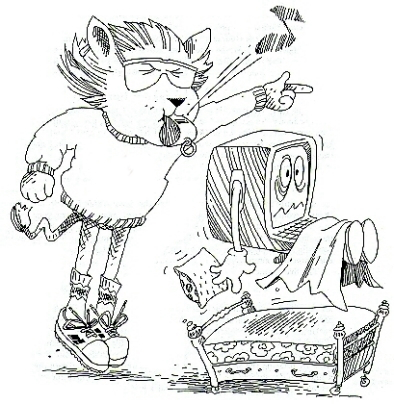
\includegraphics[width=0.4\linewidth]{figures/TexLionWhistle.jpg}
\end{frame}

\begin{frame}[fragile]
\frametitle{Codificação de arquivos}
\framesubtitle{Representação binária}
Arquivos são armazenados na forma binária no computador. 

No exemplo abaixo apresentados algumas informações sobre o arquivo \texttt{introducao.tex}
e apresentamos como é codificada a sequência de caracteres \texttt{TeX}.
\begin{footnotesize}
\begin{verbatim}
$ file introducao.tex 
introducao.tex: LaTeX document, UTF-8 Unicode text, with very long lines

$ ls -l introducao.tex
-rw-r--r-- 1 leoca leoca 9292 nov  1 14:10 introducao.tex

$ echo -n "TeX" | xxd
00000000: 5465 58                                  TeX

$ echo -n "TeX" | xxd -b
00000000: 01010100 01100101 01011000                             TeX
              T        e       X
hex          54       65      58 
dec          84      101      88
oct         124      144     130
\end{verbatim}
\end{footnotesize}
\end{frame}

\begin{frame}
\frametitle{Codificação de arquivos}
\framesubtitle{Tipos comuns de codificação}
  \begin{itemize}
  \item ASCII
  \item Windows 1252 
  \item Latin-1 (ISO-8859-1)
  \item UFT-8
  \item UTF-16
  \item UTF-32
  \end{itemize}
\end{frame}

\begin{frame}
\frametitle{Codificação de arquivos}
\framesubtitle{História}
  The Evolution of Character Codes, 1874-1968\\
  by Eric Fischer

  \vspace{2em}
  \url{https://github.com/ericfischer/ascii}
\end{frame}


\begin{frame}
\frametitle{Codificação de arquivos}
\framesubtitle{Código Morse - Samuel Morse e Alfred Vail (1837)}
        \centering
	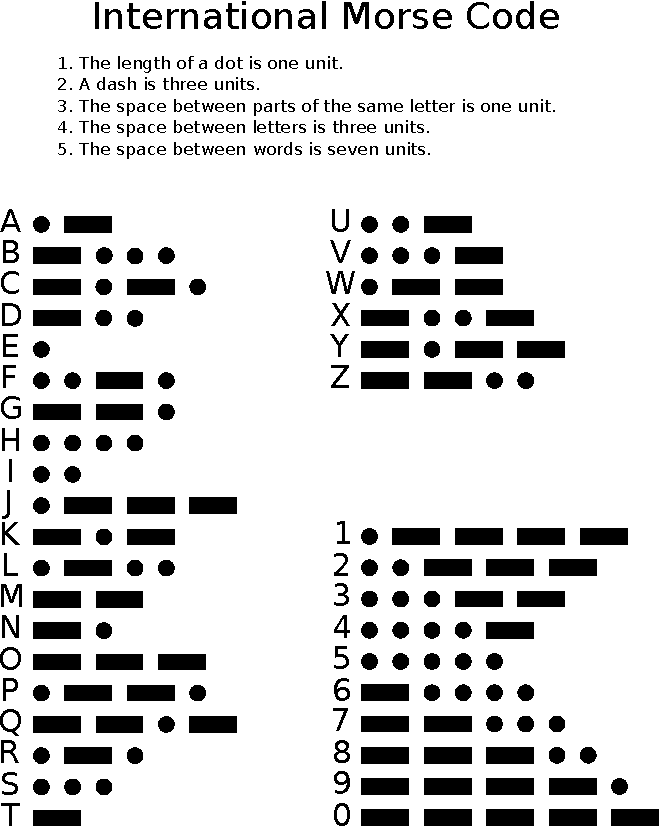
\includegraphics[width=0.3\textwidth]{figures/MorseCode.pdf} \hspace{3em}
	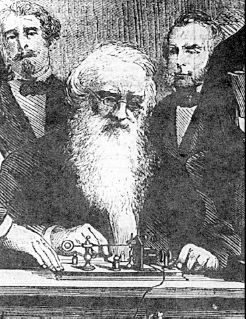
\includegraphics[width=0.3\textwidth]{figures/samuelmorse.jpg}
\end{frame}
\note{
Samuel Morse utilizou códigos de tamanho variável quando projetava o seu conhecido código telegráfico.
Samuel Morse havia sido comissionado em 1825 para pintar um retrato de Lafayette, em uma visita a Washington, DC.
Enquanto pintava, ele recebeu uma mensagem avisando que sua esposa estava muito doente.
Morse partiu imediatamente para sua casa em New Haven. Quando chegou sua esposa já havia sido enterrada.
Ele decidiu então se dedicar a explorar formas de comunicações a longa distância que fossem mais rápidas.

A primeira versão do código, desenvolvida por Morse durante uma viagem transatlântica em 1832,
era mais complexa do que a versão estabelecida em 1843. Mais tarde, Morse abandonou sua versão
em favor dos conhecidos pontos e traços desenvolvidos em conjunto com Alfred Vail.
Morse recebeu a patente do seu telégrafo com um único fio em 1847, sobrepujando o telégrafo
de múltiplos fios proposto por Cooke e Wheatstone, que havia sido patenteado em 1837.
}

\begin{frame}
\frametitle{Codificação de arquivos}
\framesubtitle{Código Baudot e Código Murray}
        \centering
	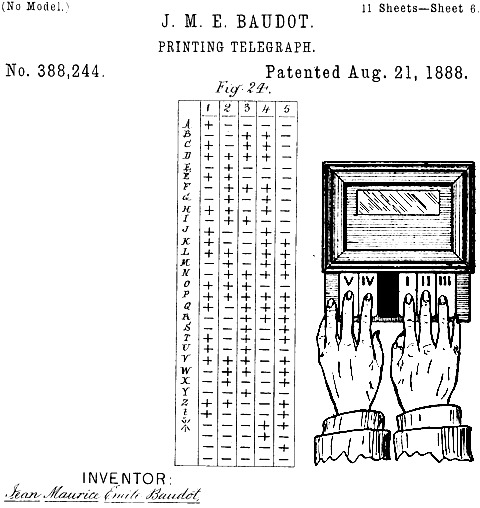
\includegraphics[width=0.3\textwidth]{figures/BaudotCode.png} \hspace{2em}
	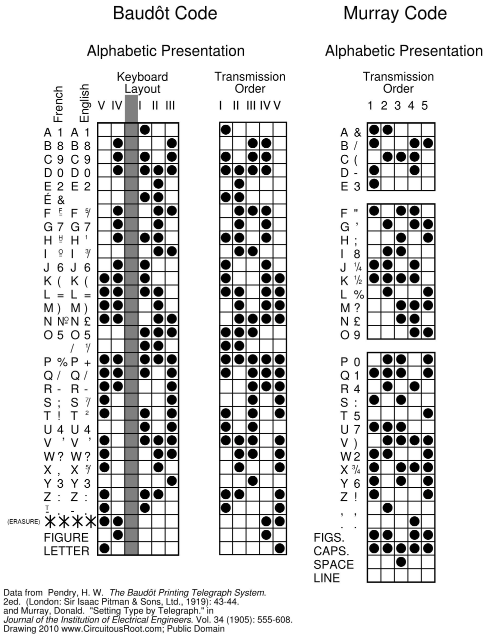
\includegraphics[width=0.35\textwidth]{figures/murraybaudot.png}
\end{frame}
\note{
Na França, Emile Baudout projetou seus sistema para o telégrafo em 1874.
Seu código foi baseado em código anterior desenvolvidos por 
Carl Friedrich Gauss e Wilhelm Weber em 1834.
Todos os símbolos possuem o mesmo comprimento, cinco. O projeto utilizava
um conjunto de fios funcionando de forma síncrona em um sistema de multiplexação,
onde o operador humano era responsável por realizar a divisão temporal e assim a sincronização.
Os códigos eram gerados por um aparelho com cinco teclas (similar às teclas de um piano),
sendo operado com duas mãos (dois dedos da mãos esquerda e três da mão direita).

Quando ordenados em alfabeticamente, as vogais e as consoantes, formam um código de Gray.

O código Baudout foi projetado para minimizar os movimentos da mão e dedos,
reduzindo assim a fadiga.
}\note{
O código de Baudout foi modificado por Donald Murray (1901) para ser utilizado
em um aparelho com teclado QWERTY. A mensagem é gravada em uma fita através de perfurações
e transmitida a partir desta fita perfurada. Deixou assim de existir a conexão direta entre
a mão do operador e a informação transmitida, não sendo mais necessário preocupar-se com a fadiga.
O objetivo passou então a ser simplificar o equipamento e minimizar seu desgaste, para tanto as
combinações com menos buracos foram utilizadas para designar caracteres mais frequentes
(ordem de freq. de occ. no inglês: e,t,a,o,i,n,s,h,r,d,l,c,u,m,w,f,g,y,p,b,v,k,j,x,q,z).


O código Murray também introduziu os caracteres de controle CR (carriage return) e
LF (line feed).
}

\begin{frame}
\frametitle{Codificação de arquivos}
\framesubtitle{Código Murray}
        \centering
        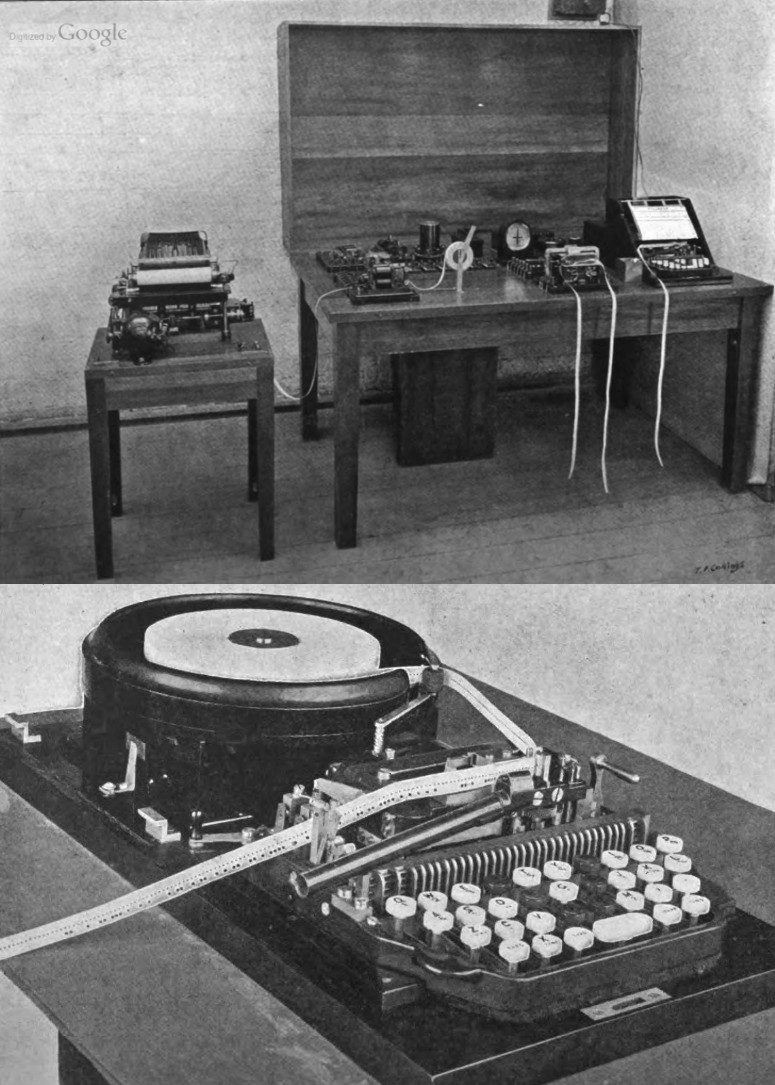
\includegraphics[width=0.35\textwidth]{figures/murrayapparatus.jpg} 
\end{frame}


\begin{frame}
\frametitle{Codificação de arquivos}
\framesubtitle{Western Union e ITA2}
   \begin{itemize}
   \item O código Murray foi adotado pelo Western Union com algumas modificações, sendo utilizado até os anos 50.
   \item Em 1924 o CCITT\footnote{O CCITT (International Telegraph and Telephone Consultative Committee) hoje conhecido
                                 como ITU-T (ITU Telecommunication Standardization Sector), um dos três setores do
                                 ITU (International Telecommunication Union) responsável pela definição de padrões em telecomunicações.}
         criou o ITA2 (international telegraph alphabet n. 2), baseado no código da Western Union.
   \item ITA2, também chamado de US TTY (American Teletypewriter code) foi a base para codificação em 5 bits dos Teletipos
         até o surgimento do código de 7 bits, ASCII em 1963.
   \end{itemize}
\end{frame}


\begin{frame}
\frametitle{Codificação de arquivos}
\framesubtitle{ASCII 1963 (7 bits)}
\centering
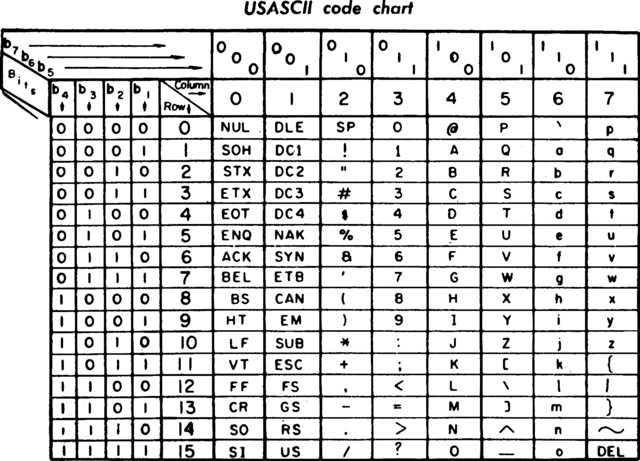
\includegraphics[width=0.65\textwidth]{figures/USASCII.png}
\end{frame}
\note{
\scriptsize
Foi desenvolvido pelo Comitê X3 da ASA (American Standards Association),
da qual faziam parte IBM (embora só passou a adotar o ASCII na década de 80),
AT\&T e sua subsidiária Teletype Corporation.

Os caracteres estão organizados de forma que os caracteres alfabéticos,
numéricos, matemáticos e de controle podem ser isolados através de uma
simples máscara binária.

O caractere A fica na posição $41_{\textmd{hex}}$ para ser compatível com o padrão
britânico. Os dígitos de 0 a 9 começam com $011$ e a sequência binária seguinte
corresponde ao valor binários de cada um deles, facilitando assim a conversão decimal-binário.

Os caracteres !"\#\$\%\&() foram adicionados à 2 coluna de forma a melhor se adequarem
à posição que ocupavam nos teclados das máquinas de escrever, de forma que a tecla \textit{shift}
corresponderia à uma simples mudança de um bit, assim facilitando a compatibilidade com as máquinas de escrever.

Foi cogitado utilizar um código com 8 bits, de forma que dois padrões de 4 bits
codificariam 2 dígitos. Isto iria requerer que fosse enviado sempre 8 bits.
Para minimizar custos, adotou-se 7 bits. Como as fitas perfuradas podiam armazenar
8 bits em cada posição, seria ainda possível utilizar um bit de paridade se desejado.
}



\begin{frame}
\frametitle{Codificação de arquivos}
\framesubtitle{Códigos de 8 bits}
  \begin{itemize}
  \item Extended ASCII 
  \item ISO/IEC 8859
  \item Windows-1252 (CP-1252)
  \end{itemize}

  Existem mais de 220 extensões DOS/Windows e 
  mais de 186 extensões EBCDIC (Extended Binary Coded Decimal Interchange Code),
  majoritariamente usado pela IBM.

  Dentre os padrões ISO o mais popular é o ISO 8859-1, também conhecido como ISO Latin 1,
  contendo a maioria dos caracteres utilizados pelas línguas da Europa Ocidental.
\end{frame}
\note{
A popularização do IBM System/360 e microprocessadores como o
Intel 8008, 8080 e 8086 acarretou na padronização do byte como uma unidade de 8 bits.
Endereçamento e armazenamento passaram a ser feitos em 8 bits, assim possibilitou a
extensão do ASCII utilizando o bit extra.
}



\begin{frame}
\frametitle{Codificação de arquivos}
\framesubtitle{Códigos Multi-Byte}
  \begin{itemize}
  \item Podem representar mais do que 256 caracteres.
  \item Alguns são extensões do ASCII (compatibilidade). Exemplo: UTF-8.
  \item UTF-16 não é uma extensão do ASCII pois os caracteres ASCII são armazenados em dois bytes, um deles igual a 0x00.
  \end{itemize}
\end{frame}


\begin{frame}[allowframebreaks]
\frametitle{Codificação de arquivos}
\framesubtitle{UFT-8}
  \begin{itemize}
  \item UTF-8: Unicode (ou Universal Coded Character Set) Transformation Format - 8-bit.
  \item Utiliza de 1 a 4 bytes.
  \item Capaz de representar até 1.112.064 pontos de codificação do Unicode.
  \item Compatibilidade reversa com ASCII (utiliza um único octeto com mesmo valor binário que o ASCII).
  \item Pontos de código mais usuais utilizam menos bytes que aqueles menos comuns.
  \item 128 caracteres ASCII necessitam de um byte (começando com 0). 
  \item 1920 caracteres utilizam 2 bytes para representar o restante do alfabeto latino (romano),
        grego, cirílico, copta, armênio, hebreu, arábico, siríaco, thaana e n'ko.
  \item Para as demais línguas são utilizados 3 bytes.
  \item 4 bytes para caracteres como símbolos matemáticos e emojis.
  \item O primeiro byte determina o número de bytes na sequência.
  \item UTF-8 foi apresentado em uma conferência em 1993. Em 2003 foi registrado pela RFC 3629 e 
        em 2008 tornou-se o padrão mais utilizado na internet.
  \item Criado por Ken Thompson e Rob Pike.
  \end{itemize}

  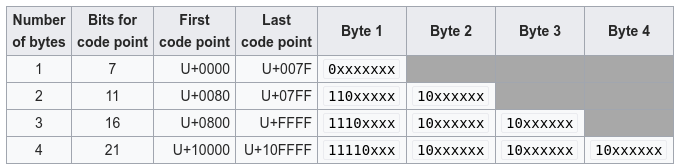
\includegraphics[width=0.85\textwidth]{figures/utf8bytes.png}

  {
  \centering
  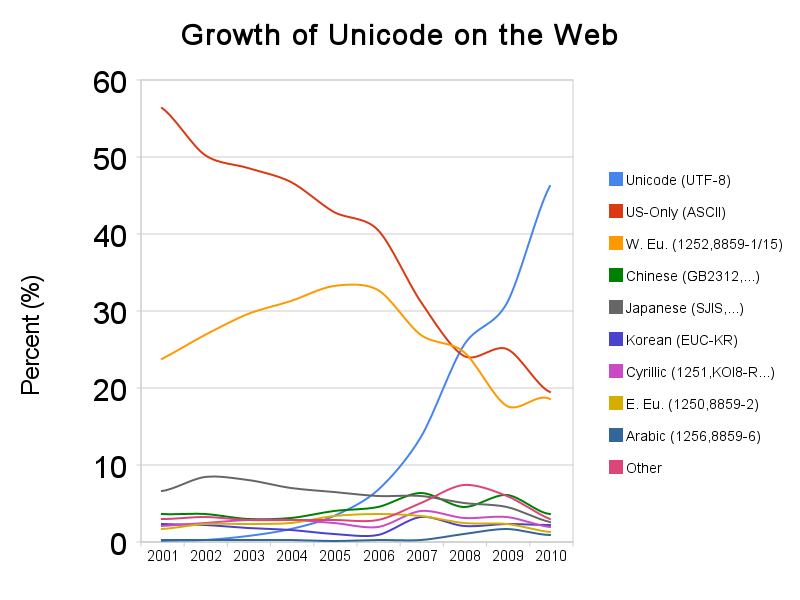
\includegraphics[width=0.55\textwidth]{figures/unicodeweb.png} 
  }
  \footnotesize{googleblog: \url{https://googleblog.blogspot.com.br/2010/01/unicode-nearing-50-of-web.html}}
  

  {
  \centering
  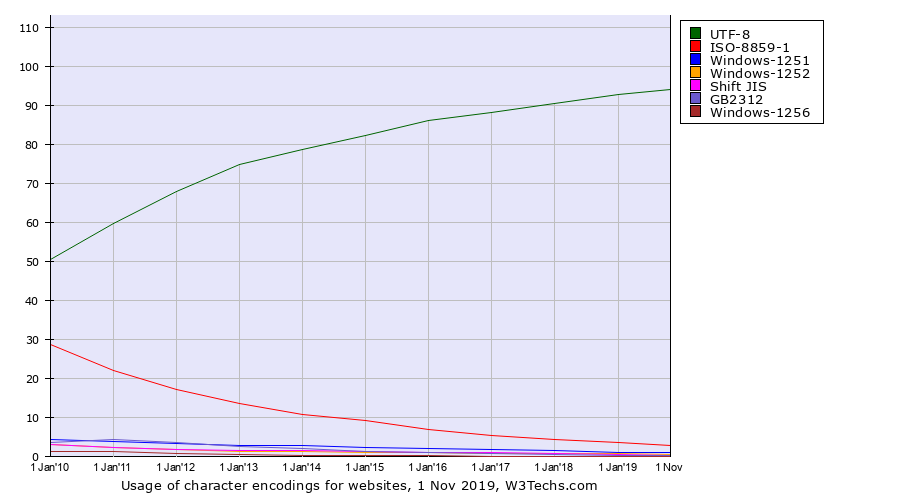
\includegraphics[width=0.6\textwidth]{figures/w3usage.png}
  }
  \footnotesize{W3Techs: \url{https://w3techs.com/technologies/history_overview/character_encoding/ms/y}}
\end{frame}


\begin{frame}
\frametitle{Codificação de arquivos}
\framesubtitle{Unicode}
  O Unicode é uma padrão para a industria de computadores para estabelecer uma 
  codificação, representação e manipulação consistente de textos utilizados por grande parte dos
  sistemas de escrita do mundo.

  A última versão do Unicode possui 136.755 caracteres cobrindo 139 escritas modernas e antigas, 
  e também outros conjuntos símbolos utilizados na comunicação humana (por exemplo, símbolos matemáticos
  e emojis).

  O Unicode é mantido pelo Consórcio do Unicode, criado em 1991, cujos membros incluem Adobe, Apple, Google, Huawei, IBM,
  Microsoft, Oracle, Yahoo! e SAP.
\end{frame}


\begin{frame}[allowframebreaks]
\frametitle{Codificação de arquivos}
\framesubtitle{Extremidade (\textit{endianness})}
  O termo \textbf{extremidade} (endianness) refere-se a ordem utilizada para armazenar/ler os bytes ou bits de dados.

  Byte 
  \hrule
  \begin{description}
  \item[big-endian]: extremidade maior primeiro -  Motorola (famílias 6800 e 68000), PowerPC (Apple).
  \item[little-endian]: extremidade menor primeiro - Intel (x86), AMD, Zilog (Z80), MOS Technology (6502), DEC (VAX e PDP-11).
  \end{description}

  Bit
  \hrule
  \begin{description}
  \item[LSB 0]: a numberação dos bits inicia-se pelo menos significante - SPARC e Motorola 68000.
  \item[MSB 0]: a numberação dos bits inicia-se pelo mais significante - S/390, PowerPC e PA-RISC (recomendada pela RfC).
  \end{description}

  \framebreak
  \begin{itemize}
  \item Lilliput - Viagens de Gulliver (Jonathan Swift).
  \item Unicode - marcador BOM (Byte Order Mark) - ponto de representação \texttt{U+FEFF}.
  \item No UTF-8 o marcador BOM é representado pela sequência de 3 octetos: \texttt{0xEF,0xBB,0xBF} (1110 1111 1011 1011 1011 1111).
  \item Extremidade (byte) é irrelevante para o padrão UTF-8 e portanto o marcador BOM é desnecessário.
  \item No padrão UTF-16 a sequência de bytes \texttt{0xFE,0xFF} indica ordenação \textit{big-endian} e a sequência \texttt{0xFF,0xFE}
        indica a ordenação \textit{little-endian}.
  \end{itemize}

\end{frame}
\note{
As CPUs que utilizam \textit{little-endian} usualmente usam o `LSB 0', enquanto
as CPUs que utilizam \textit{big-endian} utilizam ambas padronizações.
O estilo recomendado pela RfC (Request for Comments) é `MSB 0'.
Algumas arquiteturas, como SPARC e Motorola 68000 utilizam `LSB 0', enquanto
S/390, PowerPC e PA-RISC utilizam `MSB 0'.
}
\note{
``O termo em inglês para uma forma de endianness, big-endian, é uma referência às Viagens de Gulliver: 
em Lilliput houve uma guerra civil, entre os que preferiam quebrar os ovos cozidos pelo lado maior (big-endians) 
contra quem preferia quebrar os ovos cozidos pelo lado menor. Este conflito, por sua vez, era uma paródia 
entre as diferenças entre católicos e protestantes a respeito da transubstanciação.'' (Wikipedia)
\url{https://pt.wikipedia.org/wiki/Extremidade\_(ordena\\\%C3\\\%A7\\\%C3\\\%A3o)}
}


